Using different \emph{import plugins}, \sh can import data from different
sources. Currently there are plugins to import data from CSV files, SDF files
and MySQL databases bundled with the program for a more detailed description of
the plugins see \subsubsecref{subsubsec:ImportPlugins}. To perform an import you
have to  create one or more import jobs, one for each data source you want to
import. These jobs will run sequentially and the data imported by those jobs
will be merged according to rules which can be selected during the import
process. In general \sh considers two structures equal if they have the same
canonical SMILES string. If a structure is present in more than one source and properties
from these sources are mapped to the same internal property the property entries
for the structure will be merged. The following \emph{merge strategies} are
available to influence which data will be found in the finished dataset:
\label{par:importing_data_merge_strategies}
\paragraph{Do not overwrite:} The first seen occurrence of the property is used and will not be overwritten by the current job.
\paragraph{Do overwrite:} The property will be overwritten by the current import job.
\paragraph{Concatenate (only for textual properties):} The property values will
be appended at the end of the existing value.
\paragraph{Minimum / maximum (only for numeric properties):} The minimum or
maximum of the available property values will be retained.

\subsubsection{Creating Import Jobs}
\begin{figure}[ht]
   \centering
   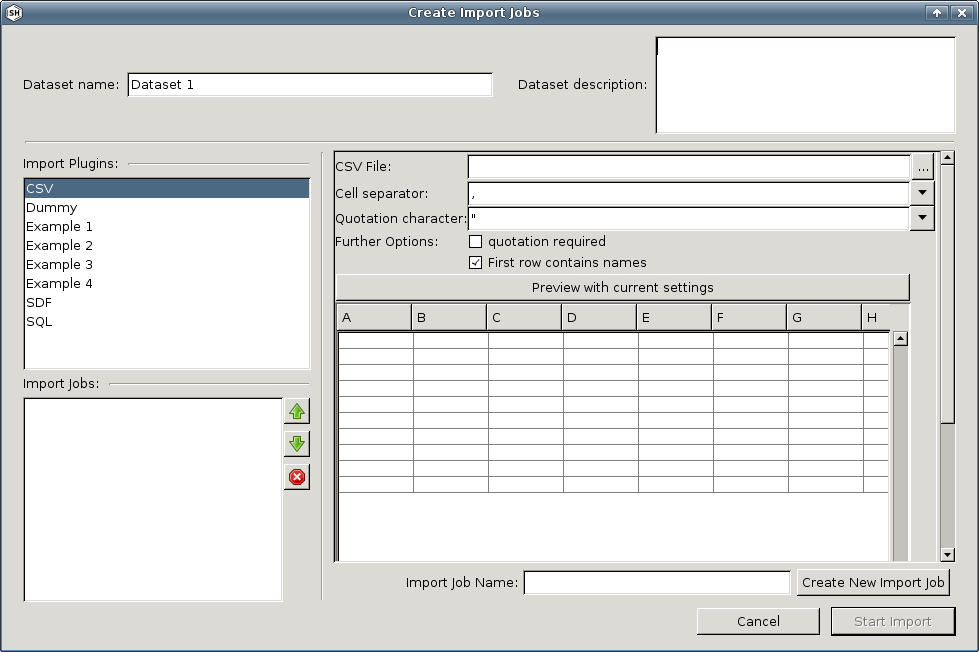
\includegraphics[width=\textwidth]{images/import/import_dialog_empty.png}
   \caption{Create Import Jobs dialog}
   \label{fig:import_dialog_empty}
\end{figure}
When you click on \gui{New Dataset} the \guidialog{Create Import Jobs} dialog
as shown in \figref{fig:import_dialog_empty} will open. In the top section
of the dialog a name and a more detailed description for the new dataset can
be entered. On the left hand side you have two lists. First the list of \gui{Import
Plugins}, where you can select a plugin appropriate for the data source you want to import.
Underneath there is the list of \gui{Import Jobs}, which contains all import
jobs created so far. The buttons beside this list can be used to delete import
jobs and to change their order. During import the jobs will be executed one after the other from top
to bottom. On the right hand side there are the settings for the currently selected plugin.
Beneath the settings you can enter an optional name for the import job. A click
on the button beside the name field will create a new import job with the
selected settings. Below this you can find a button to start the import process.

\subsubsection{Import Plugins}
\label{subsubsec:ImportPlugins}
\paragraph{CSV Import Plugin}
\begin{figure}[ht]
   \centering
   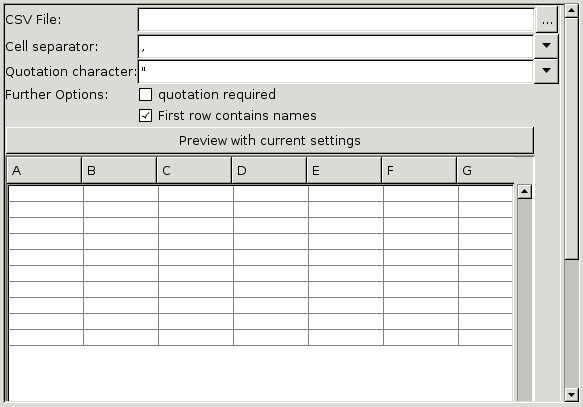
\includegraphics[width=0.5\textwidth]{images/import/csv_import_empty.png}
   \caption{CSV Import Plugin}
   \label{fig:csv_import_empty}
\end{figure} 
With the CSV plugin you can import data from comma
separated value (CSV) files. In \figref{fig:csv_import_empty} you can see
the configuration panel of the CSV plugin. You can select a CSV file, different
cell separators and quotation characters. Next to some default values you can
type in any other character. One of these options allows you to check the
\gui{quotation required} box to configure the plugin to read only quoted
content. With the \gui{First row contains names} switch you can configure the
plugin to use the first row in the CSV file for the names of the columns. If
you deselect this switch the columns will be numbered. Finally there is a
\gui{Preview with current settings} button. When you click on this button the
first 10 rows of the CSV file will be read according to your settings and
displayed in the table below. An example can be seen in
\figref{fig:csv_import_preview}.

\begin{figure}[ht]
   \centering
   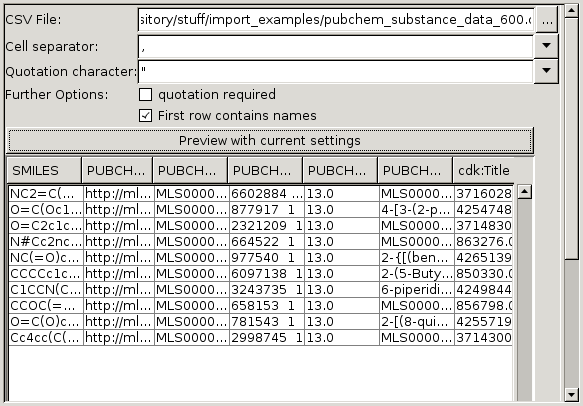
\includegraphics[width=0.5\textwidth]{images/import/csv_import_preview.png}
   \caption{CSV Import Plugin with preview}
   \label{fig:csv_import_preview}
\end{figure}

\paragraph{SQL Import Plugin}
\begin{figure}[ht]
   \centering
   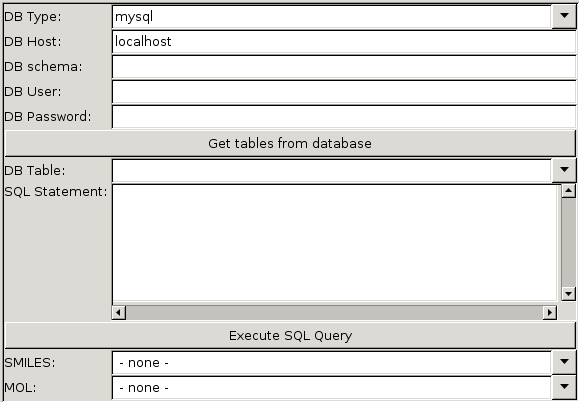
\includegraphics[width=0.5\textwidth]{images/import/sql_import_empty.png}
   \caption{SQL Import Plugin}
   \label{fig:sql_import_empty}
\end{figure}
\begin{figure}[ht]
   \centering
   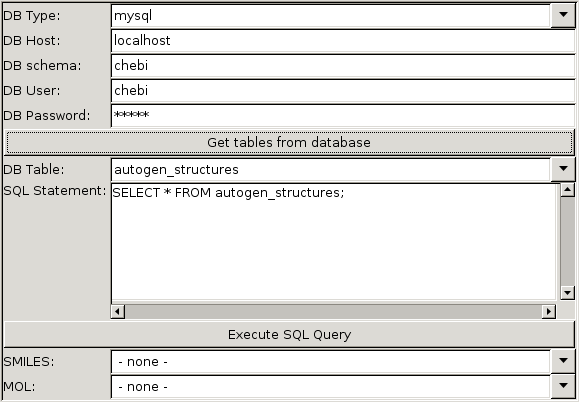
\includegraphics[width=0.5\textwidth]{images/import/sql_import_get_tables.png}
   \caption{SQL Import Plugin after \gui{Get tables from database}}
   \label{fig:sql_import_get_tables}
\end{figure}
\begin{figure}[ht]
   \centering
   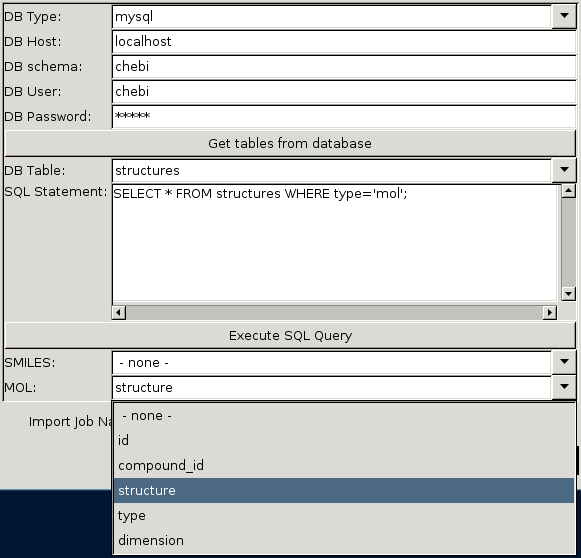
\includegraphics[width=0.5\textwidth]{images/import/sql_import_execute.png}
   \caption{SQL Import Plugin after \gui{Execute SQL Query}}
   \label{fig:sql_import_execute}
\end{figure}
The SQL import plugin allows to integrate data from SQL-based databases.
The configuration panel, as seen in \figref{fig:sql_import_empty} provides various configuration options explained in the following.
\subparagraph{DB Type}
This field allows to select the type of the SQL database you want to connect to.
Currently only \mysql is tested. Every JDBC compatible database
should be useable.  %XXX yes but they aren't
\subparagraph{DB Host}
In \gui{DB Host} you can select the database host, the server on which the source
database is running. If you need a specific port to connect to the string is: \verb+HOSTNAME:PORT+
\subparagraph{DB schema}
In the \gui{DB schema} field you can enter the database (schema) name you want to use.
\subparagraph{DB User / DB Password}
In the \gui{DB User} and \gui{DB Password} fields you can fill in your database connection credentials. Only read access is needed.
\subparagraph{Get tables from database}
Once you have entered the connection data you can click the \gui{Get tables from
database} button. The plugin will connect to the database and put all table
names found in the schema in the \gui{DB Table} list. A connection done with the ChEBI database is shown in \figref{fig:sql_import_get_tables}. 
\subparagraph{DB Table}
The \gui{DB Table} list contains the tables found after clicking on \gui{Get tables from database}. When selecting a table a  simple \verb+SELECT+ statement will be generated.
\subparagraph{SQL Statement}
In the \gui{SQL Statement} field you can type in an SQL SELECT statement that will be run on the selected database. The resulting rows from this statement will be used as source for the import.
\subparagraph{Execute SQL Query}
By clicking on \gui{Execute SQL Query} your SQL Statement will be executed and the \gui{SMILES} and \gui{MOL} lists will be filled with the resulting column names. This is shown in \figref{fig:sql_import_execute}.
\subparagraph{SMILES / MOL}
In the \gui{SMILES} and \gui{MOL} lists you can select the column names which contain structure information in SMILES and/or MOL format.

\paragraph{SDF Import Plugin}
The SDF Import plugin is very easy to use. It just has a field \gui{SDF file
name} where you enter the path to the SDF file which you want to import.

\subsubsection{Map Imported Properties Dialog}
\begin{figure}[ht]
   \centering
   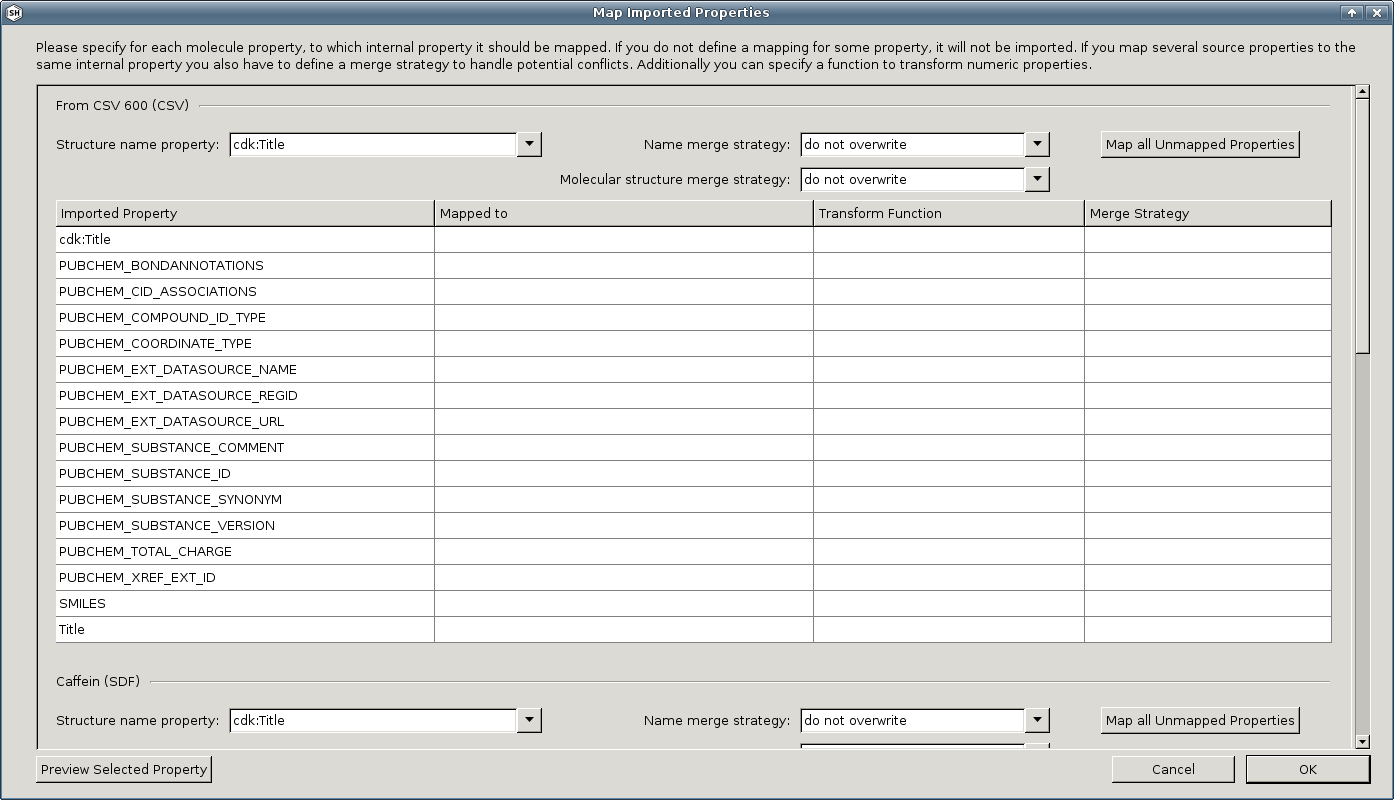
\includegraphics[width=\textwidth]{images/import/mapdialog_empty.png}
   \caption{Map Imported Properties dialog}
   \label{fig:mapdialog_empty}
\end{figure}
Once you have created at least one import job, you can start the import process
by clicking on \gui{Start Import}. A new Dialog named \gui{Map Imported
Properties} will appear. In \figref{fig:mapdialog_empty} you can see an
example of this dialog with two import jobs. For every import Job there are the
same GUI elements. At the top you have a line with the name of the following import job.
\paragraph{Structure name property}
In the \gui{Structure name property} list you select one of the properties for
the name field of the structures. The name field will be used at several places
in the program to present a name together with a structure, however it is not
used internally so there are no special requirements for this property. If the
name property is missing for some structure, the SMILES string will be used
instead.
\paragraph{Name/Molecular structure merge strategy}
In the \gui{Name merge strategy} and \gui{Molecular structure merge strategy}
you can select the merge strategies for the molecule name or 3D/2D structure
according to \parref{par:importing_data_merge_strategies}. 
\paragraph{Map all Unmapped Properties}
With the \gui{Map all Unmapped Properties} button all properties for which you
did not give  mapping information will be mapped automatically. The property
name will be the name obtained from the import plugin, the type (numeric or
text) is set also according to the plugin information as well. If multiple
sources have properties with the same name, these properties will be mapped to
the same internal property.

\hintbox{Important}{Please note that plugins typically recognize properties as
numeric only if all values of the property provided by the data source can be 
interpreted as floating point number.  As a result properties as IC$_{50}$ 
are not recognized as numeric if some values contain characters like $<$, $>$ or 
$\sim$. 
Since this may be undesirable, you may want to inspect the default mapping and
explicitly mark some properties as numeric. Values that can not be interpreted 
as floating point number will then be discarded during import.}


\paragraph{The mapping table}
In the table you have four columns. The first column (\gui{Imported Property})
shows  the property name obtained from the plugin. In the next column
(\gui{Mapped to}) you can select an existing internal property for this value,
alternatively you can choose to create a \gui{new internal property} which will
open the \gui{Create New Internal Property} Dialog (see
\subsecref{subsubsec:importing_data_create_property}) or you can choose \gui{do
not map} which will clear the table cell. In the \gui{Transform Function} column
you can input a transformation function for numerical properties, for example to
convert logarithmic to linear values. Symbols you can use are numbers, $+, -, *,
/, \verb+^+, (, ), \mathtt{log}, \mathtt{log10}, \mathtt{exp}, \mathtt{ceil}$ and
$\mathtt{floor}$. For the input value use the variable $x$. So in case you want to
convert aforementioned logarithmic values you would enter $\mathtt{exp}(x)$. In
the last column (\gui{Merge Strategy}) you can select the merge strategy for
this property. 

\paragraph{Preview Selected Property} With \gui{Preview Selected
Property} you can open a list where you can see the first 100 occurrences of the
property, which is currently selected in the table.

\subsubsection{Create New Internal Property dialog}
\label{subsubsec:importing_data_create_property}
\begin{figure}[ht]
   \centering
   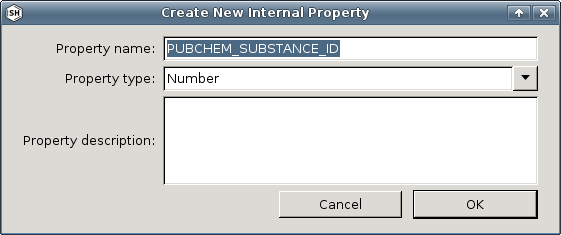
\includegraphics[width=0.5\textwidth]{images/import/create_property_empty.png}
   \caption{Create New Internal Property dialog}
   \label{fig:create_property_empty}
\end{figure}
In the \gui{Create New Internal Property} dialog, see
\figref{fig:create_property_empty} you can create new internal properties. First
you give the property a name using the \gui{Property name} field. In the
\gui{Property type} list you can select one of the property types (Number, Text, fingerprint types that can be used for clustering in the dendogram view (see \secref{sec:views:dendogram})). In \gui{Property description} you can enter a
detailed description for this property.

\subsubsection{Import into database dialog}
\begin{figure}[ht]
   \centering
   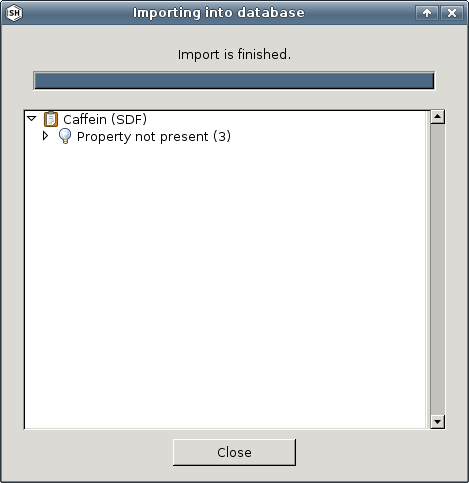
\includegraphics[width=0.5\textwidth]{images/import/import_process_finished.png}
   \caption{Importing into database dialog}
   \label{fig:import_process_finished}
\end{figure}
When you start the import in the \gui{Map Imported Properties} dialog the import
runs and the \gui{Import into database} dialog will show up. At the top you see the
current process, in the list underneath you can see some information during the
import process. When the import is finished click on \gui{Close} which concludes
creation of a new dataset.

\subsubsection{Add Properties} 
It is possible to add new properties to an existing dataset as well, by using the \gui{Add Properties} button in the \gui{Dataset and Tree Management} dialog. The process is very similar to the normal import process. However you cannot add new molecules to the dataset, due to technical reasons. Should your source contain molecules which are not contained in the current dataset, these molecules will simply be ignored during import.

Furthermore the \gui{Map Imported Properties} Dialog contains a section \gui{Merge Properties} with two fields named \gui{Source Property} and \gui{Internal Property} where you can select either to merge the datasets by molecule structure or an arbitrary property.